\chapter{\IfLanguageName{dutch}{Stand van zaken}{State of the art}}
\label{ch:stand-van-zaken}

% Tip: Begin elk hoofdstuk met een paragraaf inleiding die beschrijft hoe
% dit hoofdstuk past binnen het geheel van de bachelorproef. Geef in het
% bijzonder aan wat de link is met het vorige en volgende hoofdstuk.

% Pas na deze inleidende paragraaf komt de eerste sectiehoofding.
In deze stand van zaken worden de gebruikte technologieën stapsgewijs besproken om het nodige inzicht te creëren in het onderwerp chaos engineering. Eerst zal uitgelegd worden wat virtualisatie is en welke voordelen dit met zich meebrengt.
Vervolgens wordt toegelicht hoe softwareontwikkeling geëvolueerd is van een monolitische naar een microservices architectuur en hoe containerisatie hier een rol in speelt. Nadien zal uitleg gegeven worden over wat de containerorkestratie Kubernetes is, hoe het er voor zorgt dat applicaties dynamisch kunnen schalen en hoe er gemikt wordt naar een zo hoog mogelijke uptime ervan. Tot slot wordt besproken wat chaos engineering inhoudt en wat de link is met containerorkestratie.   

\section{Virtualisatie}

Virtualisatie maakt het mogelijk om op een fysieke computer meerdere virtuele machines uit te voeren, elk met zijn eigen besturingssysteem, geheugen, processorkernen en opslagcapaciteit.

Het essentiële onderdeel om de virtuele machines te binden aan de hardware van de fysieke host, en wat de dynamische toewijzing van resources zoals geheugen en CPU mogelijk maakt, is een softwarelaag die men de hypervisor noemt. 

\subsection{Voordelen van een hypervisor}

Het gebruik van een hypervisor om virtuele machines op een host aan te maken heeft enkele voordelen:
\begin{itemize}
    \item Snelheid: virtuele machines opzetten verloopt snel in vergelijking met de tijd benodigd om een fysieke server op te zetten.
    \item (Kost)efficiëntie: men maakt optimaal gebruik van de beschikbare resources op het hostsysteem door deze dynamisch te verdelen over meerdere virtuele machines.   
    \item Overdraagbaarheid: virtuele machines worden bewaard als bestanden op de host en zijn makkelijk overdraagbaar naar andere systemen.
\end{itemize}

\subsection{Types hypervisors}

Er bestaan twee hypervisor types:
\begin{itemize}
    \item Type 1: bare-metal / native
    \item Type 2: hosted
\end{itemize}

Een bare-metal of native type 1 hypervisor is virtualisatiesoftware die rechtstreeks geïmplementeerd is op de hardware van een host en zich gedraagt zoals een lichtgewicht besturingssysteem. Het voordeel bij dit type hypervisor is dat geen volwaardig besturingssysteem geïnstalleerd wordt en dat het hiermee gevrijwaard blijft van de kwetsbaarheden die dit met zich meebrengt. Voorbeelden van type 1 hypervisors zijn VMware ESXi, Microsoft Hyper-V, Citrix Xen ... 

Een hosted type 2 hypervisor is software die bovenop het bestaande besturingssysteem op een host aanwezig is. Het nadeel bij een type 2 hypervisor is de verhoogde latentie doordat de communicatie tussen hardware en hypervisor eerst nog het besturingsssysteem moet passeren. Bekende voorbeelden hiervan zijn de softwarepakketten VirtualBox of VMware. 

\begin{figure}[h]
    \centering
    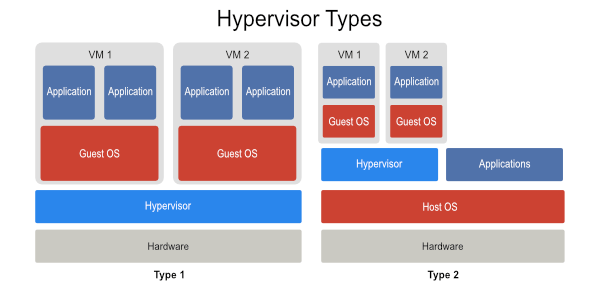
\includegraphics[scale=.6]{img/Hypervisor-Types.png}
    \caption{hypervisor types \autocite{Vembu2019}}
    \label{fig}
\end{figure}


\section{Evolutie in softwarerachitectuur}

Klassieke softwareontwikkeling leverde applicaties op die gebaseerd waren op een monolitische architectuur. Hierin was alle code aanwezig van de applicatie, zowel front- als backend. 
Dit bracht verschillende voordelen met zich mee waaronder:
\begin{itemize}
    \item makkelijk qua ontwikkeling omdat IDEs/tools gefocust waren op het bouwen van 1 applicatie.
    \item vlotter om te testen gezien de code zich allemaal in 1 applicatie bevindt. 
    \item simpel om uit te rollen in productie omdat men de verpakte applicatie slechts moest kopiëren op een server. 
    \item schalen van de applicatie eenvoudig door meerdere kopieën uit te voeren achter een load balancer.
\end{itemize} 

Verschillende nadelen van deze manier van softwarontwikkeling kwamen echter aan het licht wanneer succesvolle applicaties met de tijd begonnen te groeien. Wanneer ontwikkelaars nieuwe functionaliteit wouden toevoegen werd steeds meer code toegevoegd, waardoor de complexiteit van de applicatie steeds verhoogde. Het resultaat hiervan was dat bugs oplossen en features toevoegen steeds moeizamer verliep. Elke keer een functionaliteit veranderde aan de applicatie moest de hele applicatie opnieuw uitgerold worden, wat voor continuous deployment een enorm obstakel is.
De betrouwbaarheid van een monolitische applicatie is ook een minpunt aangezien een bug ervoor kan zorgen dat de beschikbaarheid van de volledige applicatie in het gedrang komt. \autocite{Richardson2015}

Om deze problemen met monolitische applicaties aan te pakken gebruikten grote bedrijven zoals Amazon, eBay, en Netflix een nieuwe softwareontwikkeling op basis van een microservices architectuur. Het idee achter deze nieuwe manier van softwareontwikkelling is om de applicatie op te splitsen in verschillende kleine geconnecteerde services die elk een set van features of specifieke functionaliteit bevatten.

\begin{figure}[h]
    \centering
    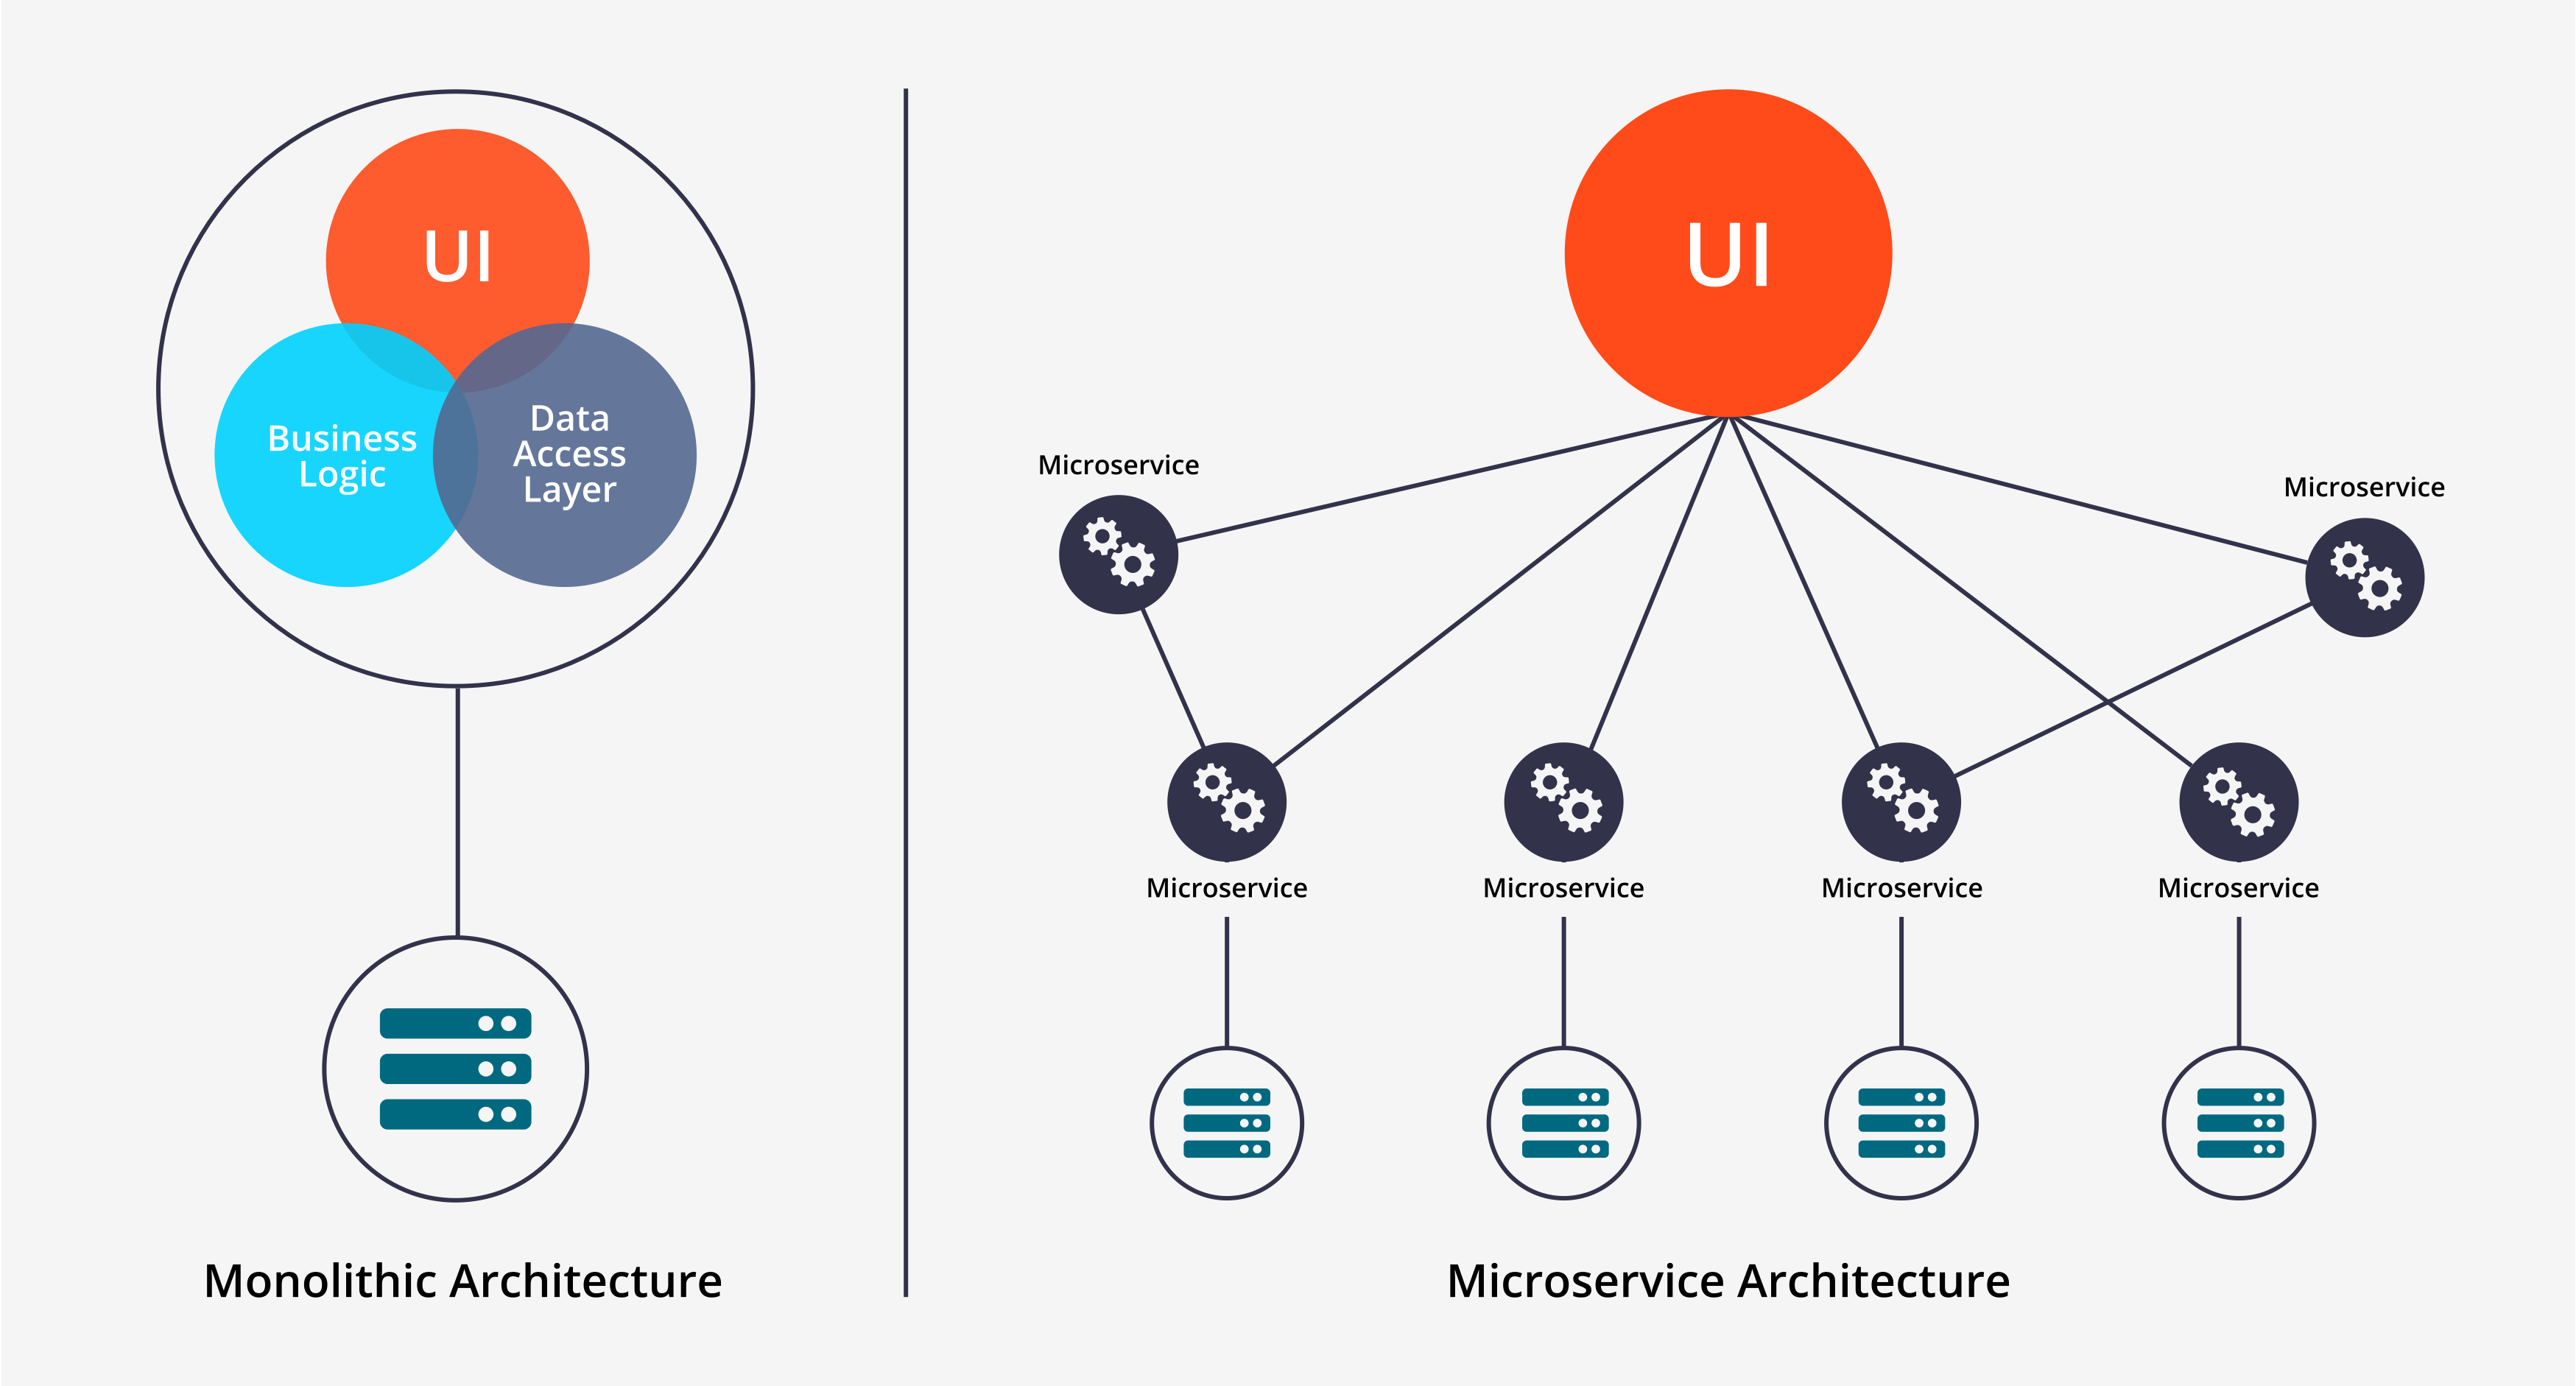
\includegraphics[scale=.1]{img/monolithic_vs_microservices.png}
    \caption{hypervisor types \autocite{Sanjaya2020}}
    \label{fig}
\end{figure}

\section{Containerisatie}

Applicaties gebouwd via een microservices architectuur brengen services onder in containers. Een container op zich bevat geen besturingssysteem maar verpakt en isoleert de code van één applicatie inclusief de gerelateerde configuratiebestanden en afhankelijkheden die deze nodig heeft. Het voordeel van containers is dat ze snel opgestart kunnen worden doordat ze weinig resources vereisen, en makkelijk overdraagbaar zijn naar verschillende omgevingen. Meerdere containers kunnen actief zijn op een systeem en maken ook allemaal gebruik van hetzelfde besturingssysteem. \autocite{Singh2020}

Ondanks dat containers net zoals virtuele machines een vorm van virtualisatie zijn, is er toch een belangrijk onderscheid te maken. Containers zijn namelijk een vorm van besturingssysteemvirtualisatie, dit tegenover virtuele machines die aan hardwarevirtualisatie doen.
Hierdoor verbruiken containers dus minder resources ten opzichte van virtuele machines. \autocite{Holt2018}

Containers en virtuele machines kunnen gecombineerd worden om virtuele omgevingen te maken waarin software ontwikkeld en getest kan worden. Containers blijven wel afhankelijk van het besturingssysteem. Men kan geen Windows containers in een Linux omgeving opstarten of omgekeerd. Om de interactie met het besturingssysteem op de host mogelijk te maken is een container runtime op het systeem nodig zoals Docker Engine, CRI-O, LXC ...

\subsection{Docker}

De oorsprong van containers kan herleid worden naar 1979 toen men voor het eerst een proces kon isoleren via de system call chroot in Unix V7. Pas vanaf 2000 kwamen bedrijven zoals Open Virtuzzo en Google met nieuwe ontwikkellingen zoals cgroups en LXC (Linux containers) die de concepten rond containerisatie meer vorm begonnen te geven. Het was pas echter toen Docker in 2013 op de markt kwam dat het gebruik van containers qua populariteit explodeerde. 
Docker maakte het onderscheid door een volledig ecosysteem aan te bieden voor container management.\autocite{Osnat2020} 

Door Docker Engine op het systeem te installeren kan men gecontaineriseerde applicaties op gelijk welke infrastructuur uitvoeren. Voordien kon men hinder ondervinden doordat afhankelijkheden van applicaties ervoor zorgden dat het uitvoeren ervan in een andere omgeving problemen kon geven. Dit probleem wordt vaak omschreven als de 'dependency hell'.

Met Docker bundelt een ontwikkelaar een applicatie en zijn afhankelijkheden in een container die overal uitvoerbaar is. Om een applicatie in een container te plaatsen is een Dockerfile nodig. 
Dit bestand plaatst men bij de applicatie en is in essentie een set instructies waarin de applicatiecode inclusief de benodigde afhankelijkheden gekopieerd worden naar de container en hoe de applicatie opgestart wordt. De Dockerfile zal vervolgens gebruikt worden om een image te maken, die opgeslagen wordt in een publieke repository zoals Docker Hub of een private repository.

Wanneer men de applicatie op een ander systeem wil opbouwen, waar Docker ook geïnstalleerd is, kan men via het docker run commando de image van de applicatie uit een repository halen en hiermee een container op het systeem lanceren die de applicatie bevat.  

\section{Containerorkestratie}

In een productieomgeving moet men ervoor zorgen dat applicaties continu beschikbaar blijven en deze fouttolerant zijn. Wanneer een container faalt, moet een andere container automatisch opgestart worden om dit op te vangen. Wanneer meer gebruik gemaakt wordt van een applicatie, moet deze automatisch kunnen schalen om deze extra vraag op te vangen. Om deze redenen en nog veel meer wordt containerorkestratie toegepast.

Containerorkestratie is het volledige proces rond het uitrollen, beheren en schalen van gecontaineriseerde applicaties. De bekendste speler in containerorchestratie is ongetwijfeld Kubernetes (K8s). Andere aanbieders in deze markt zijn o.a. Nomad, Docker Swarm, Amazon Elastic Kubernetes Service (EKS) ...
Bij het opzetten van de verschillende virtuele omgevingen die later in hoofdstuk 3 uitvoerig besproken worden werd enkel gebruik gemaakt van Kubernetes.

\subsection{Kubernetes} 

Ongeveer 1 jaar nadat de containerisatiesoftware Docker in 2013 op de markt verscheen, werd Kubernetes aan het grote publiek voorgesteld. Oorspronkelijk werd het ontwikkeld door Google, maar nu wordt het project onderhouden door de Cloud Native Computing Foundation (https://www.cncf.io/).

Kubernetes wordt op hun eigen website omschreven als een overdraagbaar, uit te breiden, open-source platform voor het beheer van gecontaineriseerde applicaties en services, dat zowel declaratieve als geautomatiseerde configuratie toelaat.

\subsection{Kubernetes architectuur}

Het grootste object in de Kubernetes architectuur noemt men een cluster. Hierin worden fysieke of virtuele machines als nodes gegroepeerd. Men kan afhankelijk van het aantal nodes twee types clusters onderscheiden:
\begin{itemize}
    \item een single-node cluster 
    \item een multi-node cluster 
\end{itemize} 
 
Wanneer men meerdere nodes in een cluster onderbrengt kan het onderscheid gemaakt worden tussen:
\begin{itemize}
    \item de control-plane node(s)
    \item de worker node(s)
\end{itemize} 
In een single-node cluster is de enige node zowel de control-plane als worker node. 

De control-plane node(s) zijn verantwoordelijk voor het beheren van de worker nodes. Op de worker nodes zullen de containers geplaatst worden van een applicatie. Een container wordt ondergebracht in een Pod, wat het kleinste Kubernetes object is. 

Een Pod kan meer dan 1 container bevatten, maar nooit van dezelfde aard. XXXXXXX

Kubernetes bevat een aantal componenten die afhankelijk van het type node zullen geïnstalleerd worden. Op deze manier zijn de verantwoordelijkheden in een cluster duidelijk afgelijnd. De volgende componenten ziet men in elke cluster terugkeren: 
\begin{itemize}
    \item API server: de front-end voor de control-plane en laat interactie met een cluster toe. 
    \item etcd: een key-value store die gebruikt wordt om clusterdata op te slaan. 
    \item scheduler: verantwoordelijk voor de distributie van containers naar de nodes.
    \item controller: verantwoordelijk voor het monitoren en reageren wanneer nodes/pods uitvallen. De controller beslist als nieuwe nodes/pods gecreërd moeten worden.
    \item container runtime: de onderliggende software die het mogelijk maakt om containers uit te voeren bv. Docker   
    \item kubelet: een agent die op elke node actief is en verantwoordelijk is voor de correcte uitvoering van de containers.   
\end{itemize}

\subsection{Helm}

Een besturingssysteem maakt vaak standaard gebruik van een pakketbeheerder (of package manager). Denk maar aan apt bij de Linux distributie Debian, of yum bij distributie Red Hat Enterprise Linux. Dit maakt het mogelijk om software te (de)installeren en softwareupgrades uit te voeren.

Ook Kubernetes maakt gebruik van een eigen package manager genaamd Helm, die het mogelijk maakt om Kubernetes applicaties te beheren. Via Helm charts kan men de meest complexe Kubernetes applicaties definiëren, installeren en upgraden.

Later in dit onderzoek, tijdens de installatie van de lokale Kubernetes distributie KinD zal Helm gebruikt worden. 

\section{Chaos Engineering}
  
Dit hoofdstuk bevat je literatuurstudie. De inhoud gaat verder op de inleiding, maar zal het onderwerp van de bachelorproef *diepgaand* uitspitten. De bedoeling is dat de lezer na lezing van dit hoofdstuk helemaal op de hoogte is van de huidige stand van zaken (state-of-the-art) in het onderzoeksdomein. Iemand die niet vertrouwd is met het onderwerp, weet nu voldoende om de rest van het verhaal te kunnen volgen, zonder dat die er nog andere informatie moet over opzoeken \autocite{Pollefliet2011}.

Je verwijst bij elke bewering die je doet, vakterm die je introduceert, enz. naar je bronnen. In \LaTeX{} kan dat met het commando \texttt{$\backslash${textcite\{\}}} of \texttt{$\backslash${autocite\{\}}}. Als argument van het commando geef je de ``sleutel'' van een ``record'' in een bibliografische databank in het Bib\LaTeX{}-formaat (een tekstbestand). Als je expliciet naar de auteur verwijst in de zin, gebruik je \texttt{$\backslash${}textcite\{\}}.
Soms wil je de auteur niet expliciet vernoemen, dan gebruik je \texttt{$\backslash${}autocite\{\}}. In de volgende paragraaf een voorbeeld van elk.

\textcite{Knuth1998} schreef een van de standaardwerken over sorteer- en zoekalgoritmen. Experten zijn het erover eens dat cloud computing een interessante opportuniteit vormen, zowel voor gebruikers als voor dienstverleners op vlak van informatietechnologie~\autocite{Creeger2009}.

\lipsum[7-20]
